\section{Discretization of the Mat\'ern SPDE}
\label{sec:discretization_matern}

In the following analysis we consider a 2D field
$\uni(\x)$, $\x\in\openBdy$ since this is
relevant to our control parameters, although we note that the
extension to 3D is relatively straightforward.
We carry out the discretization on a structured nonuniform grid according to the
finite volume method - as is the general setting in the MITgcm.
We note that our development is similar to \citet{fuglstad_exploring_2015},
who show a differential operator for a 2D field on a uniform grid.

Figure \ref{fig:mitgcm_grid} shows the general structure of the grid, and
defines the various grid cell distances used in the derivation.
We begin by integrating equation (\ref{eq:spde_general}),
\begin{linenomath}\begin{equation}
    \begin{aligned}
        \int_{\openBdy} \delta(\x)\,\uni(\x)\, d\x -
        \int_{\openBdy} \nabla\cdot K(\x)\nabla\,\uni(\x)\,d\x
        &=
        \int_{\openBdy} \W(\x)\defdet^{-1/2} \, d\x \\
        \sum_{\jk}\int_{\cell_\jk} \delta(\x)\,\uni(\x)\, d\x -
        \sum_{\jk}\int_{\cell_\jk} \nabla\cdot K(\x)\nabla\,\uni(\x)\,d\x
        &=
        \sum_{\jk}\int_{\cell_\jk} \W(\x)\defdet^{-1/2} \, d\x \, ,
    \end{aligned}
    \label{eq:spde_integral}
\end{equation}\end{linenomath}
where in second line we distribute the integral across each grid cell
$\cell_\jk\subset\openBdy$.

\begin{figure}
    \centering
    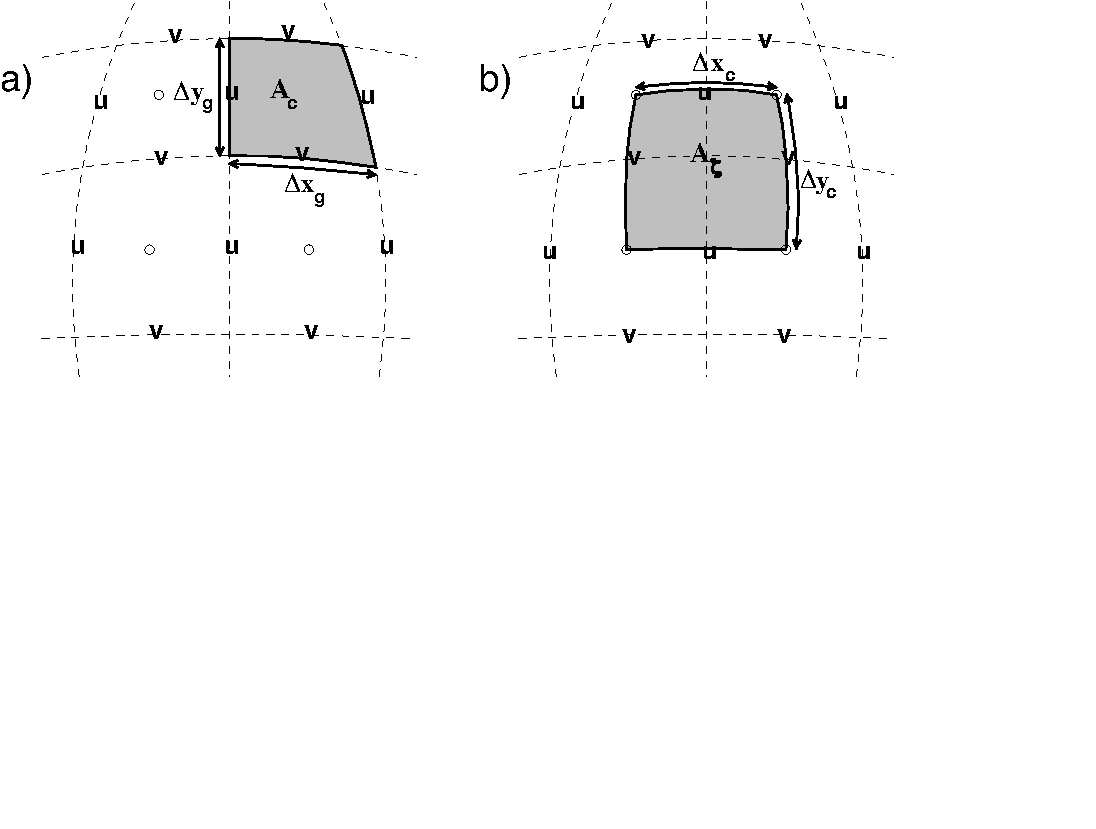
\includegraphics[width=.6\textwidth]{../figures/hgrid-abcd.pdf}
    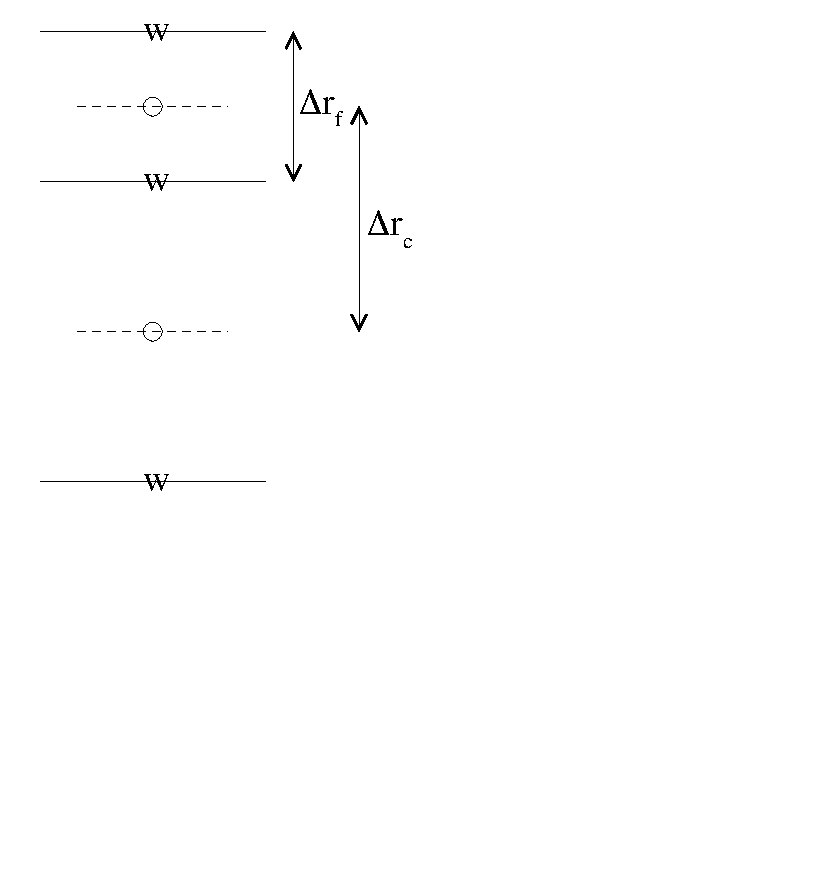
\includegraphics[width=.2\textwidth]{../figures/vgrid-accur-center.pdf}
    \caption{The structured finite volume grid used in the MITgcm. The
        left two figures show the horizontal grid, viewed from above. The right
        figure shows the vertical grid. In each figure, u, v, and w mark the
        location where velocities exist on the grid cell interfaces. The open
        circles denote the tracer location at the grid cell center,
        where fields like temperature and salinity are located. Figures are from
    \citet{campin_mitgcmmitgcm_2021}.}
    \label{fig:mitgcm_grid}
\end{figure}

Starting with the first term,
\begin{linenomath*}\begin{equation*}
    \delta_\jk \coloneqq \dfrac{1}{\vol_\jk}\int_{\cell_\jk}\delta(\x)\,d\x
\end{equation*}\end{linenomath*}
so that
\begin{linenomath*}\begin{equation*}
    \int_{\cell_\jk} \delta(\x)\,\uni(\x)\, d\x =
    \vol_\jk\,\delta_\jk\,\uni_\jk
\end{equation*}\end{linenomath*}
where $\vol_\jk = \Delta y^{j}_{g} \Delta r_f^k$ is the grid cell volume,
indicated by Figure \ref{fig:mitgcm_grid}.
We note that a cartesian style notation
is used, but spherical polar coordinates are used in the computation, and the
MITgcm supports generic curvilinear coordinates.
Generally, the coordinate directions $(x,y,z)$ correspond to $(\lambda,\phi,r)$,
i.e. longitude, latitude, and height.
In the spherical polar case, the differential elements are
\begin{linenomath*}\begin{equation*}
    \Delta x = r_0 \cos(\phi)\Delta\lambda \qquad
    \Delta y = r_0 \Delta \phi \qquad
    \Delta z = \Delta r
\end{equation*}\end{linenomath*}
where $r_0 = 6,378$ km is the nominal radius of the earth, and note that in this
coordinate system latitude $\phi$ is defined to be 0 at the equator.

The third term is, from the definition of a white noise process
\citep{adler_random_2007},
\begin{linenomath*}\begin{equation*}
    \int_{\cell_\jk}\defdet^{-1/2}\W(\x) \, d\x
        = \sqrt{\dfrac{\vol_\jk}{\defdetd}} z_\jk
\end{equation*}\end{linenomath*}
where $z_\jk$ is an uncorrelated (independent) standard Gaussian at each grid
cell center $\jk$, and we used:
\begin{linenomath*}\begin{equation*}
    \defdetd \coloneqq
    \dfrac{1}{\vol_\jk}\int_{\cell_\jk}\defdet\,d\x\,.
\end{equation*}\end{linenomath*}

The second term, containing the Laplacian is handled as follows
\begin{linenomath*}\begin{equation*}
    \int_{\cell_\jk} \nabla\cdot K(\x)\nabla\,\uni(\x)\,d\x
    =\int_{\cellbdy_\jk} K(\x)\nabla\,\uni(\x)\,
    \cdot \hat{\mathbf{n}} \, d\s
\end{equation*}\end{linenomath*}
where $\hat{\mathbf{n}}$ is an outward normal to the cell boundary
$\cellbdy_\jk$.
Throughout this work, we assume the tensor $K(\x)$ to be represented as the
diagonal matrix:
\begin{linenomath*}\begin{equation*}
    K(\x) =
    \begin{pmatrix}
        \kappa^{vy}(\x) & 0 \\
        0 & \kappa^{wz}(\x) \\
    \end{pmatrix} \, .
\end{equation*}\end{linenomath*}
Our choice here is discussed later, and could be generalized in future work.
We represent the
discretized form of this tensor as
\begin{linenomath*}\begin{equation*}
    K_\jk =
    \begin{pmatrix}
        \kappa^{vy}_\jk & 0 \\
        0 & \kappa^{wz}_\jk \\
    \end{pmatrix} \, ,
\end{equation*}\end{linenomath*}
where the elements $\kappa^{vy}_\jk$ and $\kappa^{wz}_\jk$
are located at the $v$ and $w$ grid cell locations in Figure
\ref{fig:mitgcm_grid}.
Additionally
\begin{linenomath*}\begin{equation*}
    \kappa^{vy}_{\jk} \coloneqq \dfrac{1}{\Delta r_f^{\jk}}
    \int_{\cellbdy_{\jk}^{S}} \kappa^{vy}(\x)\,d\x
    \qquad
    \kappa^{wz}_{\jk} \coloneqq \dfrac{1}{\Delta y_g^{\jk}}
    \int_{\cellbdy_{\jk}^{B}} \kappa^{wz}(\x)\,d\x
\end{equation*}\end{linenomath*}
where $\cellbdy_{\jk}^{S}$ and $\cellbdy_{\jk}^{B}$ are the
southern and bottom boundaries of the grid cell.
The discretized gradient is approximated via the finite difference
directional derivative at each cell face:
\begin{linenomath*}\begin{equation*}
    \begin{aligned}
%        \pderiv{\uni}{x}(\x_\jk^W)
%        &\simeq \dfrac{\uni_\jk - \uni_\imjk}{\Delta x_c^\jk}
%        \qquad
%        \pderiv{\uni}{x}(\x_\jk^E)
%        &&\simeq \dfrac{\uni_\ipjk - \uni_\jk}{\Delta x_c^\ipjk}
%        \\
        \pderiv{\uni}{y}(\x_\jk^S)
        &\simeq \dfrac{\uni_\jk - \uni_\jmk}{\Delta y_c^\jk}
        \qquad
        \pderiv{\uni}{y}(\x_\jk^N)
        &&\simeq \dfrac{\uni_\jpk - \uni_\jk}{\Delta y_c^\jpk}
        \\
        \pderiv{\uni}{z}(\x_\jk^B)
        &\simeq \dfrac{\uni_\jk - \uni_\jkm}{\Delta z_c^\jk}
        \qquad
        \pderiv{\uni}{z}(\x_\jk^T)
        &&\simeq \dfrac{\uni_\jkp - \uni_\jk}{\Delta z_c^\jkp}
    \end{aligned}
\end{equation*}\end{linenomath*}
for the south, north, bottom, and top cell faces, respectively.
Putting these definitions together,
\begin{linenomath}\begin{equation}
    \begin{aligned}
        \int_{\cellbdy_\jk}
        &K(\x)\nabla\,\uni(\x)\,
        \cdot \hat{\mathbf{n}} \, d\s
        \coloneqq \\
%        &\left[
%            \left(
%            \dfrac{\kappa^{ux} \, \Delta y_g \Delta r_f}{\Delta x_c}
%            \right)_\ipjk \,
%            (\uni_\ipjk - \uni_\jk) -
%            \left(
%            \dfrac{\kappa^{ux} \, \Delta y_g \Delta r_f}{\Delta x_c}
%            \right)_\jk \,
%            (\uni_\jk - \uni_\imjk)
%        \right]+
%        \\
        &\left[
            \left(
            \dfrac{\kappa^{vy} \, \Delta r_f}{\Delta y_c}
            \right)_\jpk \,
            (\uni_\jpk - \uni_\jk) -
            \left(
            \dfrac{\kappa^{vy} \, \Delta r_f}{\Delta y_c}
            \right)_\jk \,
            (\uni_\jk - \uni_\jmk)
        \right]+
        \\
        &\left[
            \left(
            \dfrac{\kappa^{wz} \, \Delta y_g}{\Delta r_c}
            \right)_\jkp \,
            (\uni_\jkp - \uni_\jk) -
            \left(
            \dfrac{\kappa^{wz} \, \Delta y_g}{\Delta r_c}
            \right)_\jk \,
            (\uni_\jk - \uni_\jkm)
        \right]
        \, .
    \end{aligned}
    \label{eq:big_laplacian}
\end{equation}\end{linenomath}
With each term in equation \eqref{eq:spde_integral} defined above, we have the system of
equations in matrix form:
\begin{linenomath}\begin{equation}
    \begin{aligned}
        (D_\delta - L) \unis &= D_z\mathbf{z}\\
        A\unis &= D_z\mathbf{z}
    \end{aligned}
    \label{eq:fv_spde}
\end{equation}\end{linenomath}
where we have (left) divided by grid cell volume so that:
\begin{linenomath*}\begin{equation*}
    \begin{aligned}
        D_\delta \coloneqq \text{diag}\{\delta_i\}_{i=1}^{\nuni} \qquad
        D_z \coloneqq \text{diag}\left\{
            \dfrac{1}{\sqrt{\vol_i \,\, \defdetdi}}
            \right\}_{i=1}^{\nuni}
    \end{aligned}
\end{equation*}\end{linenomath*}
where for notational simplicity we index each grid cell with $i$, rather than
$j$ and $k$ as above.
Finally, $L$ is defined by appropriately gathering terms in
equation \eqref{eq:big_laplacian}, applying the boundary conditions discussed in the next
subsection, and left dividing by grid cell volume.

At last, the covariance matrix associated with the vector $\unis$ can be
obtained by considering the joint probability distribution of
$\mathbf{z}\sim\mathcal{N}(0,I)$ and
the relation $\mathbf{z} = D_z^{-1}A\unis$, obtained from
equation \eqref{eq:fv_spde}.
That is,
\begin{linenomath*}\begin{equation*}
    \begin{aligned}
        \pi(\mathbf{z})
        &\propto  \exp\left\{-\dfrac{1}{2}\mathbf{z}^T\mathbf{z}\right\} \\
        &\propto \exp\left\{-\dfrac{1}{2}\unis^T A D_z^{-2} A \unis\right\} \\
        &\propto \pi(\unis) \, ,
    \end{aligned}
\end{equation*}\end{linenomath*}
where we note that $A=A^T$.
Thus, we define the differential operator for our covariance model as
\begin{linenomath*}\begin{equation*}
    C \coloneqq A^{-1} D_z \, .
\end{equation*}\end{linenomath*}
\\

\noindent\textbf{Neumann boundary conditions.}
So far we have omitted the discussion of boundaries for the sake of
simplicity.
We employ the Neumann boundary condition:
\begin{linenomath*}\begin{equation*}
    K(\x)\nabla\uni(\x) \cdot \hat{\mathbf{n}} = 0 \qquad \x\in\groundBdy \, .
\end{equation*}\end{linenomath*}
which are implemented in equation \eqref{eq:big_laplacian}
simply by zeroing out the gradient term at solid boundaries.
We note that this has an impact on the covariance structure that is discussed
more concretely with the numerical results in
section \ref{sec:matern_pig}.\\

\noindent\textbf{Generic form of the covariance.}
With the Mat\'ern covariance operator $C$ defined, we recall that
\begin{linenomath*}\begin{equation*}
    \Gamma_{\uni} = \Gamma_{\uni}^{1/2}\Gamma_{\uni}^{T/2}
    = \Sigma X C C^T X \Sigma \, ,
\end{equation*}\end{linenomath*}
and all that is left to define are the operators $X$ and $\Sigma$.
We reserve the definition of $\Sigma$ to
chapter xx, as this becomes somewhat specific to our
application.
Recall that $X$ is defined through the pointwise marginal variance of the
covariance operator $C$.
This can feasibly be computed as $\mathbf{e}_i^TCC^T\mathbf{e}_i$, with
$\mathbf{e}_i$ being the canonical basis vector associated with the $i$th
element of the grid.
However, we compute an approximation based on samples from the covariance model, as
suggested in \citet{weaver_correlation_2001} (and references therein).
Samples of the Gaussian random variable with mean $\unis_0$ and covariance
$C C^T$ are computed as
\begin{linenomath*}\begin{equation*}
    \unis = \unis_0 + C\mathbf{z} \, .
\end{equation*}\end{linenomath*}
We find $X$ by computing the standard deviation from a sample size of $N=1000$.
We note that using this approach to approximate the variance of $C$ scales well
to higher dimensional applications.
Additionally, this approach fits well into our computational framework, since
computing these random samples is a necessary first step for the randomized
eigenvalue decomposition algorithm that is fundamental to our inference problem.
